% $Header: /cvsroot/latex-beamer/latex-beamer/solutions/conference-talks/conference-ornate-20min.en.tex,v 1.6 2004/10/07 20:53:08 tantau Exp $

\documentclass{beamer}

% This file is a solution template for:

% - Talk at a conference/colloquium.
% - Talk length is about 20min.
% - Style is ornate.



% Copyright 2004 by Till Tantau <tantau@users.sourceforge.net>.
%
% In principle, this file can be redistributed and/or modified under
% the terms of the GNU Public License, version 2.
%
% However, this file is supposed to be a template to be modified
% for your own needs. For this reason, if you use this file as a
% template and not specifically distribute it as part of a another
% package/program, I grant the extra permission to freely copy and
% modify this file as you see fit and even to delete this copyright
% notice. 


\mode<presentation>
{
  \usetheme{Madrid}
  % or ...

  \setbeamercovered{transparent}
  % or whatever (possibly just delete it)
}


\usepackage[english]{babel}
% or whatever

\usepackage[latin1]{inputenc}
% or whatever

\usepackage{times}
\usepackage[T1]{fontenc}
% Or whatever. Note that the encoding and the font should match. If T1
% does not look nice, try deleting the line with the fontenc.
\usepackage{url}
\usepackage{epstopdf}


\title
{Practical GRIDportal}

\subtitle
{Working with mpiBLAST} % (optional)

\author
{Martin Matusiak}
% - Give the names in the same order as the appear in the paper.
% - Use the \inst{?} command only if the authors have different
%   affiliation.

\institute[NTNU HPC Project]
{
  The NTNU High Performance Computing Project\\
  Norwegian University of Science and Technology
}
% - Use the \inst command only if there are several affiliations.
% - Keep it simple, no one is interested in your street address.

\date % (optional, should be abbreviation of conference name)
{10 November 2005}
% - Either use conference name or its abbreviation.
% - Not really informative to the audience, more for people (including
%   yourself) who are reading the slides online


% Delete this, if you do not want the table of contents to pop up at
% the beginning of each subsection:
\AtBeginSection[]
{
  \begin{frame}<beamer>
    \frametitle{Outline}
    \tableofcontents[currentsection,currentsubsection]
  \end{frame}
}


% If you wish to uncover everything in a step-wise fashion, uncomment
% the following command: 

%\beamerdefaultoverlayspecification{<+->}


\begin{document}

\begin{frame}
  \titlepage
\end{frame}

\begin{frame}
  \frametitle{Outline}
  \tableofcontents
  % You might wish to add the option [pausesections]
\end{frame}


% Structuring a talk is a difficult task and the following structure
% may not be suitable. Here are some rules that apply for this
% solution: 

% - Exactly two or three sections (other than the summary).
% - At *most* three subsections per section.
% - Talk about 30s to 2min per frame. So there should be between about
%   15 and 30 frames, all told.

% - A conference audience is likely to know very little of what you
%   are going to talk about. So *simplify*!
% - In a 20min talk, getting the main ideas across is hard
%   enough. Leave out details, even if it means being less precise than
%   you think necessary.
% - If you omit details that are vital to the proof/implementation,
%   just say so once. Everybody will be happy with that.

\section{Introducing GRIDportal}




%\subsection{The command line interface}



\begin{frame}
  \frametitle{GRID: a network of computer resources}

	\begin{center}
		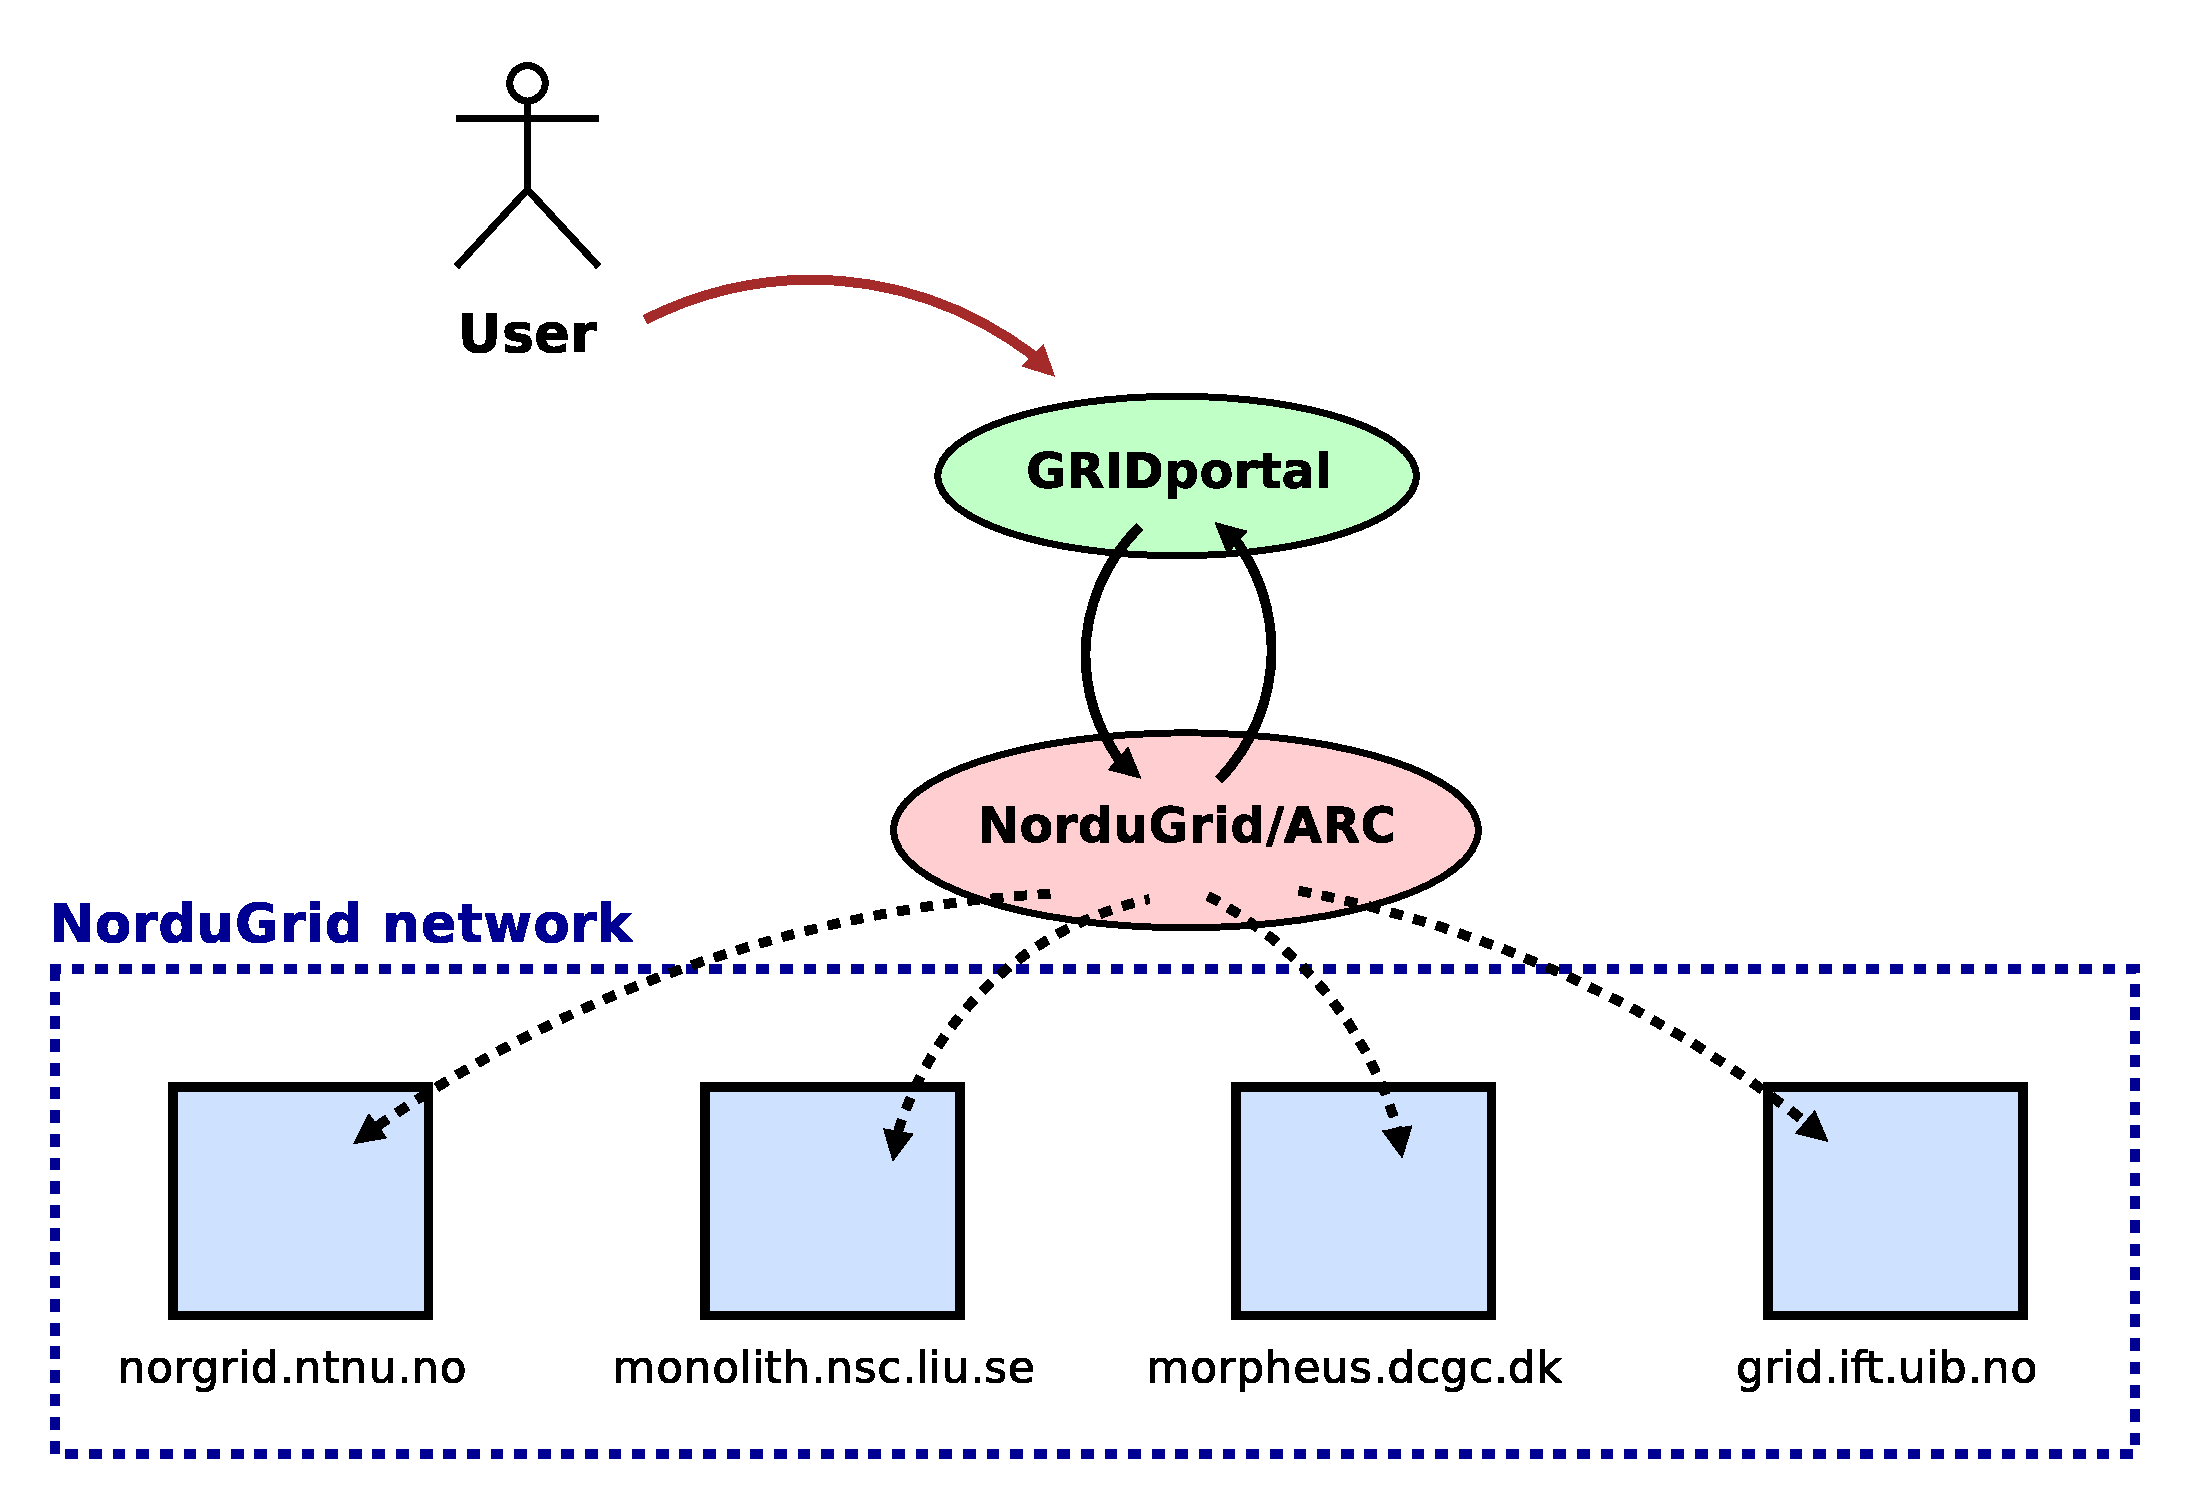
\includegraphics[width=0.86\textwidth]{nordugrid.eps}
	\end{center}
\end{frame}

\begin{frame}
  \frametitle{A quick look at NorduGrid/ARC}

	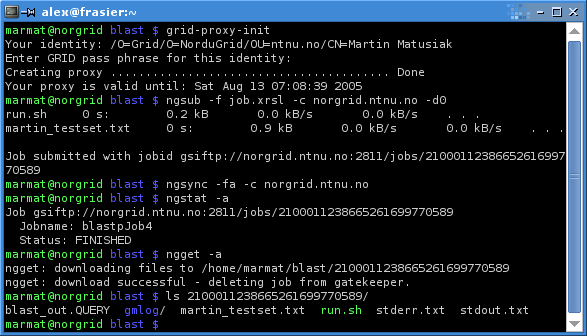
\includegraphics[width=\textwidth]{console_submit.png}
\end{frame}

\begin{frame}
  \frametitle{GRIDportal: a web-based grid application portal}

	\begin{center}
		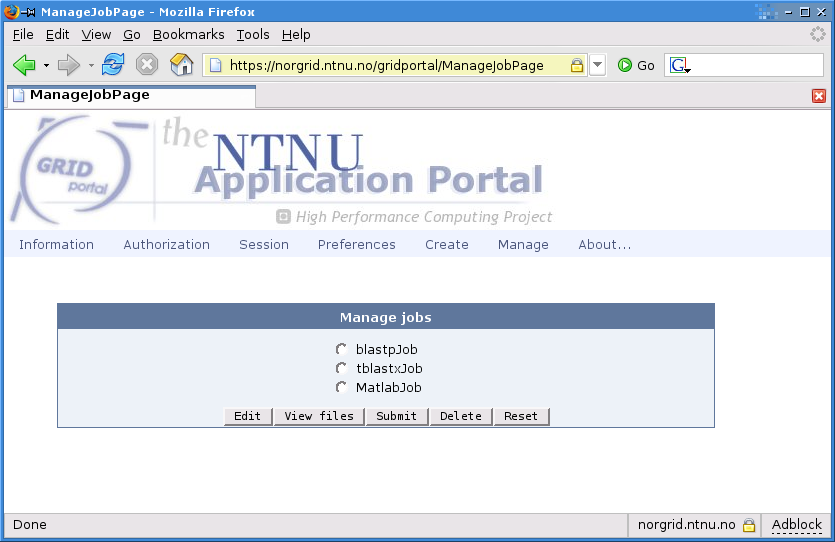
\includegraphics[width=0.9\textwidth]{gridportal_managejobs.png}
	\end{center}
\end{frame}







\section{Working with mpiBLAST}







\begin{frame}
  \frametitle{What is mpiBLAST?}

	A flavor of BLAST designed to run on a cluster (a number of computers [nodes] connected together). {\bf BLAST and mpiBLAST are near identical in use.}\\
	\bigskip
	The way mpiBLAST works is that it
  \begin{enumerate}
  	\item divides the database into equal segments,
  	\item distributes each segment onto a node,
  	\item performs BLAST search on each node in parallell,
  	\item and merges the results from each node into a common result set.
  \end{enumerate}
\end{frame}

\begin{frame}
  \frametitle{Creating a BLAST job}

	\begin{center}
		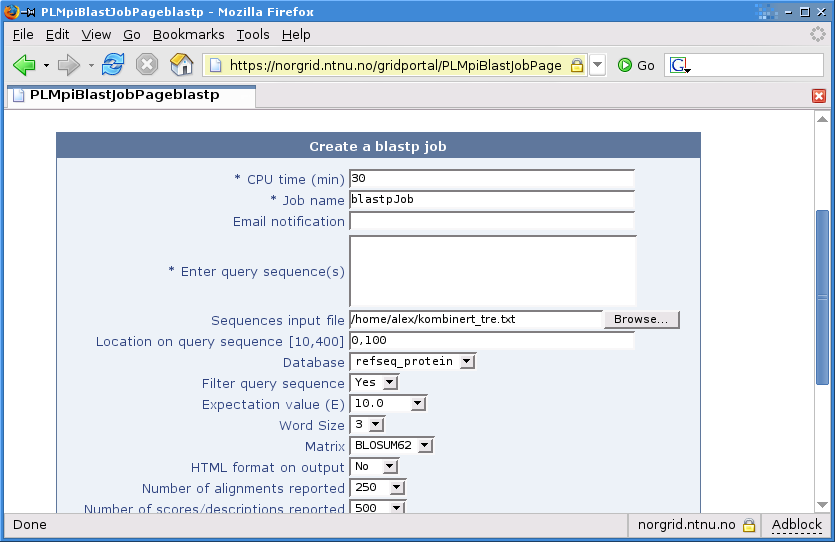
\includegraphics[width=0.9\textwidth]{gridportal_createblast.png}
	\end{center}
\end{frame}

\begin{frame}
  \frametitle{Submitting a BLAST job}

	\begin{center}
		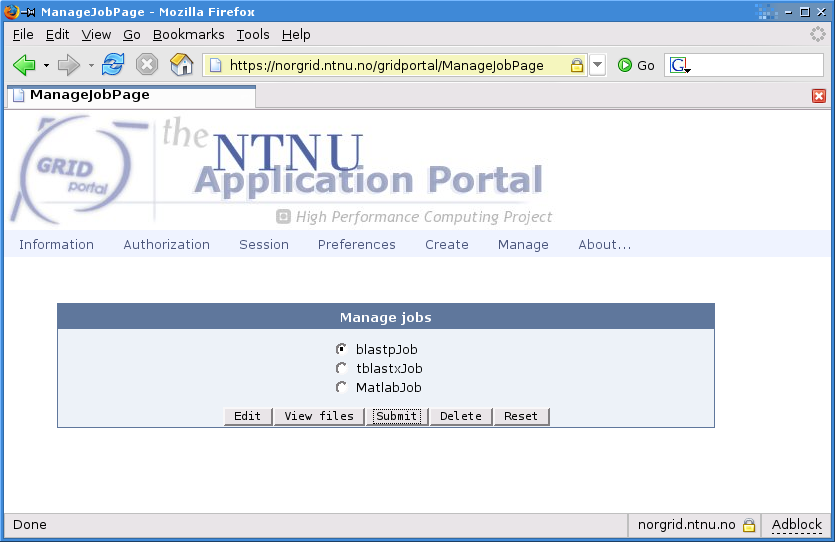
\includegraphics[width=0.9\textwidth]{gridportal_submitjob.png}
	\end{center}
\end{frame}

\begin{frame}
  \frametitle{Checking up on a job}

	\begin{center}
		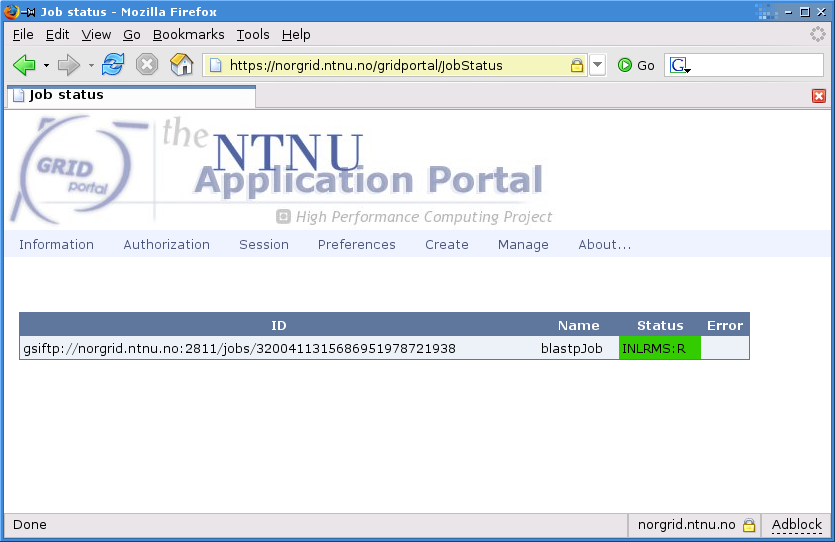
\includegraphics[width=0.9\textwidth]{gridportal_jobstatus.png}
	\end{center}
\end{frame}

\begin{frame}
  \frametitle{Getting job results}

	\begin{center}
		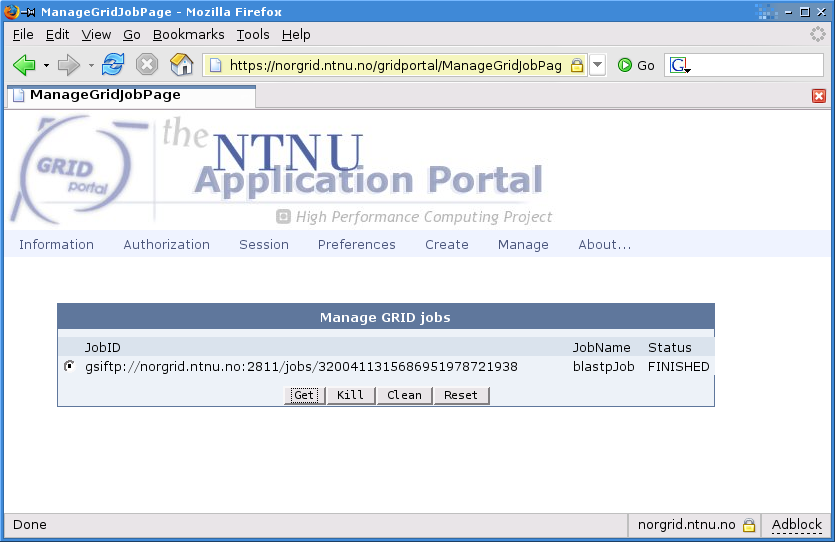
\includegraphics[width=0.9\textwidth]{gridportal_getjob.png}
	\end{center}
\end{frame}

\begin{frame}
  \frametitle{Viewing results of a job}

	\begin{center}
		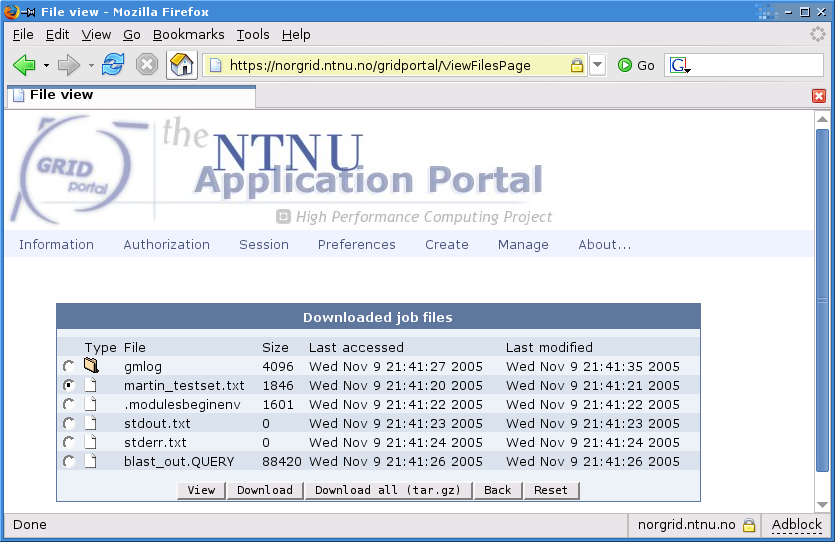
\includegraphics[width=0.9\textwidth]{gridportal_jobviewfiles.png}
	\end{center}
\end{frame}

\begin{frame}
  \frametitle{Viewing job files}

	\begin{center}
		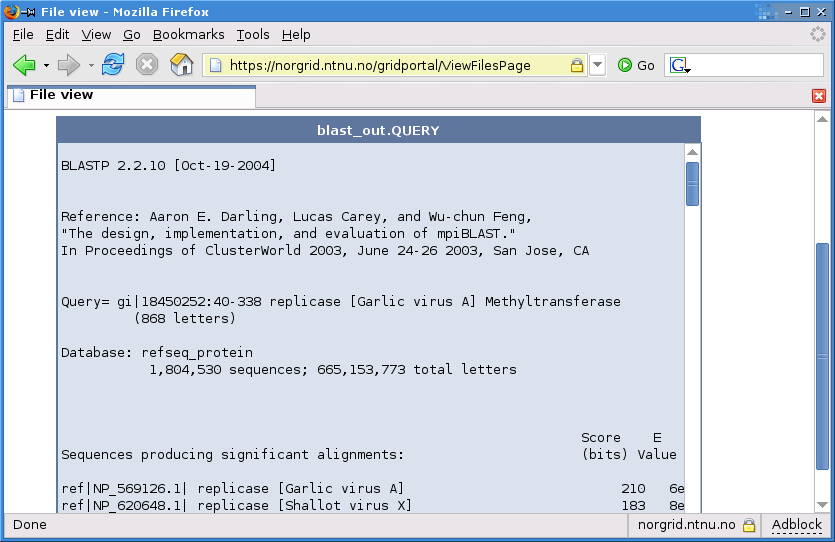
\includegraphics[width=0.9\textwidth]{gridportal_jobviewfile.png}
	\end{center}
\end{frame}



\appendix
\section<presentation>*{\appendixname}
\subsection<presentation>*{References}

\begin{frame}
  \frametitle{Links}

  \begin{itemize}
  	\item GRIDportal project website <\url{http://gridportal.dynalias.org/}>
  	\item GRIDportal deployment site <\url{http://norgrid.ntnu.no/gridportal/}>
  \end{itemize}
  \bigskip

  \begin{center}
  Thank you for your attention!
  \end{center}
\end{frame}




\end{document}


